\PassOptionsToPackage{unicode=true}{hyperref} % options for packages loaded elsewhere
\PassOptionsToPackage{hyphens}{url}
%
\documentclass[12pt,]{article}
\usepackage{lmodern}
\usepackage{amssymb,amsmath}
\usepackage{ifxetex,ifluatex}
\usepackage{fixltx2e} % provides \textsubscript
\ifnum 0\ifxetex 1\fi\ifluatex 1\fi=0 % if pdftex
  \usepackage[T1]{fontenc}
  \usepackage[utf8]{inputenc}
  \usepackage{textcomp} % provides euro and other symbols
\else % if luatex or xelatex
  \usepackage{unicode-math}
  \defaultfontfeatures{Ligatures=TeX,Scale=MatchLowercase}
    \setmainfont[]{Times New Roman}
\fi
% use upquote if available, for straight quotes in verbatim environments
\IfFileExists{upquote.sty}{\usepackage{upquote}}{}
% use microtype if available
\IfFileExists{microtype.sty}{%
\usepackage[]{microtype}
\UseMicrotypeSet[protrusion]{basicmath} % disable protrusion for tt fonts
}{}
\IfFileExists{parskip.sty}{%
\usepackage{parskip}
}{% else
\setlength{\parindent}{0pt}
\setlength{\parskip}{6pt plus 2pt minus 1pt}
}
\usepackage{hyperref}
\hypersetup{
            pdftitle={Central Appalachian Mine Closures},
            pdfauthor={Hannah Smith},
            pdfborder={0 0 0},
            breaklinks=true}
\urlstyle{same}  % don't use monospace font for urls
\usepackage[margin=2.54cm]{geometry}
\usepackage{color}
\usepackage{fancyvrb}
\newcommand{\VerbBar}{|}
\newcommand{\VERB}{\Verb[commandchars=\\\{\}]}
\DefineVerbatimEnvironment{Highlighting}{Verbatim}{commandchars=\\\{\}}
% Add ',fontsize=\small' for more characters per line
\usepackage{framed}
\definecolor{shadecolor}{RGB}{248,248,248}
\newenvironment{Shaded}{\begin{snugshade}}{\end{snugshade}}
\newcommand{\AlertTok}[1]{\textcolor[rgb]{0.94,0.16,0.16}{#1}}
\newcommand{\AnnotationTok}[1]{\textcolor[rgb]{0.56,0.35,0.01}{\textbf{\textit{#1}}}}
\newcommand{\AttributeTok}[1]{\textcolor[rgb]{0.77,0.63,0.00}{#1}}
\newcommand{\BaseNTok}[1]{\textcolor[rgb]{0.00,0.00,0.81}{#1}}
\newcommand{\BuiltInTok}[1]{#1}
\newcommand{\CharTok}[1]{\textcolor[rgb]{0.31,0.60,0.02}{#1}}
\newcommand{\CommentTok}[1]{\textcolor[rgb]{0.56,0.35,0.01}{\textit{#1}}}
\newcommand{\CommentVarTok}[1]{\textcolor[rgb]{0.56,0.35,0.01}{\textbf{\textit{#1}}}}
\newcommand{\ConstantTok}[1]{\textcolor[rgb]{0.00,0.00,0.00}{#1}}
\newcommand{\ControlFlowTok}[1]{\textcolor[rgb]{0.13,0.29,0.53}{\textbf{#1}}}
\newcommand{\DataTypeTok}[1]{\textcolor[rgb]{0.13,0.29,0.53}{#1}}
\newcommand{\DecValTok}[1]{\textcolor[rgb]{0.00,0.00,0.81}{#1}}
\newcommand{\DocumentationTok}[1]{\textcolor[rgb]{0.56,0.35,0.01}{\textbf{\textit{#1}}}}
\newcommand{\ErrorTok}[1]{\textcolor[rgb]{0.64,0.00,0.00}{\textbf{#1}}}
\newcommand{\ExtensionTok}[1]{#1}
\newcommand{\FloatTok}[1]{\textcolor[rgb]{0.00,0.00,0.81}{#1}}
\newcommand{\FunctionTok}[1]{\textcolor[rgb]{0.00,0.00,0.00}{#1}}
\newcommand{\ImportTok}[1]{#1}
\newcommand{\InformationTok}[1]{\textcolor[rgb]{0.56,0.35,0.01}{\textbf{\textit{#1}}}}
\newcommand{\KeywordTok}[1]{\textcolor[rgb]{0.13,0.29,0.53}{\textbf{#1}}}
\newcommand{\NormalTok}[1]{#1}
\newcommand{\OperatorTok}[1]{\textcolor[rgb]{0.81,0.36,0.00}{\textbf{#1}}}
\newcommand{\OtherTok}[1]{\textcolor[rgb]{0.56,0.35,0.01}{#1}}
\newcommand{\PreprocessorTok}[1]{\textcolor[rgb]{0.56,0.35,0.01}{\textit{#1}}}
\newcommand{\RegionMarkerTok}[1]{#1}
\newcommand{\SpecialCharTok}[1]{\textcolor[rgb]{0.00,0.00,0.00}{#1}}
\newcommand{\SpecialStringTok}[1]{\textcolor[rgb]{0.31,0.60,0.02}{#1}}
\newcommand{\StringTok}[1]{\textcolor[rgb]{0.31,0.60,0.02}{#1}}
\newcommand{\VariableTok}[1]{\textcolor[rgb]{0.00,0.00,0.00}{#1}}
\newcommand{\VerbatimStringTok}[1]{\textcolor[rgb]{0.31,0.60,0.02}{#1}}
\newcommand{\WarningTok}[1]{\textcolor[rgb]{0.56,0.35,0.01}{\textbf{\textit{#1}}}}
\usepackage{graphicx,grffile}
\makeatletter
\def\maxwidth{\ifdim\Gin@nat@width>\linewidth\linewidth\else\Gin@nat@width\fi}
\def\maxheight{\ifdim\Gin@nat@height>\textheight\textheight\else\Gin@nat@height\fi}
\makeatother
% Scale images if necessary, so that they will not overflow the page
% margins by default, and it is still possible to overwrite the defaults
% using explicit options in \includegraphics[width, height, ...]{}
\setkeys{Gin}{width=\maxwidth,height=\maxheight,keepaspectratio}
\setlength{\emergencystretch}{3em}  % prevent overfull lines
\providecommand{\tightlist}{%
  \setlength{\itemsep}{0pt}\setlength{\parskip}{0pt}}
\setcounter{secnumdepth}{5}
% Redefines (sub)paragraphs to behave more like sections
\ifx\paragraph\undefined\else
\let\oldparagraph\paragraph
\renewcommand{\paragraph}[1]{\oldparagraph{#1}\mbox{}}
\fi
\ifx\subparagraph\undefined\else
\let\oldsubparagraph\subparagraph
\renewcommand{\subparagraph}[1]{\oldsubparagraph{#1}\mbox{}}
\fi

% set default figure placement to htbp
\makeatletter
\def\fps@figure{htbp}
\makeatother

\usepackage{etoolbox}
\makeatletter
\providecommand{\subtitle}[1]{% add subtitle to \maketitle
  \apptocmd{\@title}{\par {\large #1 \par}}{}{}
}
\makeatother

\title{Central Appalachian Mine Closures}
\providecommand{\subtitle}[1]{}
\subtitle{\url{https://github.com/hgs13/EDA_Final_Project_2020}}
\author{Hannah Smith}
\date{}

\begin{document}
\maketitle

\newpage
\tableofcontents 
\newpage
\listoftables 
\newpage
\listoffigures 
\newpage

\hypertarget{rationale-and-research-questions}{%
\section{Rationale and Research
Questions}\label{rationale-and-research-questions}}

This project seeks to analyze the migration patterns of residents of
coal counties in central Appalachia from the years 2000 to 2017. Two
``coal counties'' serve as a case study for migration in central
Appalachia: Harlan County, Kentucky and Dickenson County, Virginia.
Harlan County serves as a ``Boom Bust'' county, meaning the county
experienced a coal production boom in 2000 and a coal production bust in
2010. Dickenson, on the other hand, is a ``Bust Bust'' county, where the
county experienced a coal production bust in 2000 and did not recover by
2010.

An important portion of understanding migration in Appalachia is
investigating the mine operations within the coal counties. As such,
this project creates and analyzes a visualization of mine production and
employee in Harlan and Dickenson counties between the years 2000 and
2011. The data analysis of the coal production and the number of
employees in coal mines in each county could be indicative of migration
patterns within the central Appalachian region.

\newpage

\hypertarget{dataset-information}{%
\section{Dataset Information}\label{dataset-information}}

The data in this repository is coal mine data compiled by the Coal and
America Bass Connections team at Duke University from the Energy
Information Administration (EIA) online database throughout the fall of
2019. The data in this repository is coal mine data compiled by the Coal
and America Bass Connections team at Duke University from the Energy
Information Administration (EIA) online database throughout the fall of
2019.

"This report is mandatory under the Federal Energy Administration Act of
1974 (Public Law 93-275). Failure to comply may result in criminal
fines, civil penalties, and other sanctions as provided by law. Title 18
USC 1001 makes it a criminal offense for any person knowingly and
willingly to make to any Agency or Department of the United States any
false, fictitious, or fraudulent statements as to any matter within its
jurisdiction.

All coal mining companies that owned a mining operation which produced
25,000 or more short tons of coal during the reporting year must submit
form EIA-7A, except for anthracite mines. All anthracite mines that
produced 10,000 or more short tons during the reporting year must submit
form EIA-7A. Standalone facilities (e.g., preparation
plant/tipple/loading dock/train loadout) that worked 5,000 or more hours
must submit the EIA-7A. Submit a separate form EIA-7A for each mining
operation and standalone facility that meets the reporting criteria.

The U.S. Energy Information Administration's (EIA) Form EIA-7A, Annual
Survey of Coal Production and Preparation, collects coal production data
from U.S. coal mining companies. This includes information on the type
and status of coal operations, characteristics of coalbeds mined,
recoverable reserves, productive capacity and the disposition of coal
mined which provides Congress with basic statistics concerning coal
supply. These data appear in the Annual Coal Report, the Quarterly Coal
Report, the Monthly Energy Review, and the Annual Energy Review. In
addition, the EIA uses the data for coal supply analyses and in
short-term modeling efforts, which produce forecasts of coal supply and
prices requested by Congress. The forecast data also appear in the
Short-Term Energy Outlook and the Annual Energy Outlook."

Therefore, the data used in this project should be timely and accurate.
Furthermore, coal production during the decade this project explores was
extremely variable. As such, there should be no exclusion of outliers in
this report.

\newpage

\hypertarget{exploratory-analysis}{%
\section{Exploratory Analysis}\label{exploratory-analysis}}

\hypertarget{data-exploration}{%
\subsection{Data Exploration}\label{data-exploration}}

Data exploration of the Harlan and Dickenson County raw data files.

\begin{Shaded}
\begin{Highlighting}[]
\KeywordTok{dim}\NormalTok{(harlan.raw)}
\end{Highlighting}
\end{Shaded}

\begin{verbatim}
## [1] 509  15
\end{verbatim}

\begin{Shaded}
\begin{Highlighting}[]
\KeywordTok{dim}\NormalTok{(dickenson.raw)}
\end{Highlighting}
\end{Shaded}

\begin{verbatim}
## [1] 194  15
\end{verbatim}

\begin{Shaded}
\begin{Highlighting}[]
\KeywordTok{str}\NormalTok{(harlan.raw)}
\end{Highlighting}
\end{Shaded}

\begin{verbatim}
## 'data.frame':    509 obs. of  15 variables:
##  $ year                     : int  2011 2011 2011 2011 2011 2011 2011 2011 2011 2011 ...
##  $ mine.name                : Factor w/ 126 levels "# 1","# 2","# 3",..: 34 104 122 46 41 91 47 14 86 39 ...
##  $ mine.state               : Factor w/ 1 level "Kentucky (East)": 1 1 1 1 1 1 1 1 1 1 ...
##  $ countystr                : Factor w/ 1 level "Harlan": 1 1 1 1 1 1 1 1 1 1 ...
##  $ mine.basin               : Factor w/ 1 level "Appalachia Central": 1 1 1 1 1 1 1 1 1 1 ...
##  $ mine.status              : Factor w/ 6 levels "Active","Active, men not working, not producing",..: 1 1 1 1 1 1 1 1 1 1 ...
##  $ mine.type                : Factor w/ 1 level "Underground": 1 1 1 1 1 1 1 1 1 1 ...
##  $ company.type             : Factor w/ 3 levels "Contractor","Indepedent Producer Operator",..: 2 2 2 2 2 2 2 2 2 2 ...
##  $ operation.type           : Factor w/ 2 levels "Mine only","Preparation Plant": 1 2 2 2 2 2 1 2 1 2 ...
##  $ operating.company        : Factor w/ 102 levels "A & M Coal Co Inc",..: 54 64 37 37 31 76 54 69 46 54 ...
##  $ operating.company.address: Factor w/ 92 levels "1160 Jackson Dr, Paris, TN 38242",..: 33 21 59 59 58 50 33 48 57 33 ...
##  $ production.stons         : Factor w/ 400 levels "0","1,013,140",..: 248 1 1 1 1 1 313 1 81 1 ...
##  $ average.employees        : int  110 25 22 20 2 9 127 2 35 4 ...
##  $ labor.hours              : Factor w/ 468 levels "","1,211","1,692",..: 174 243 365 380 302 92 193 298 446 8 ...
##  $ ARC                      : int  1 1 1 1 1 1 1 1 1 1 ...
\end{verbatim}

\begin{Shaded}
\begin{Highlighting}[]
\KeywordTok{str}\NormalTok{(dickenson.raw)}
\end{Highlighting}
\end{Shaded}

\begin{verbatim}
## 'data.frame':    194 obs. of  15 variables:
##  $ year                     : int  2011 2011 2011 2011 2011 2011 2011 2011 2011 2011 ...
##  $ mine.name                : Factor w/ 56 levels "#1","#2","#44",..: 37 16 36 32 11 10 17 6 50 55 ...
##  $ mine.state               : Factor w/ 1 level "Virginia": 1 1 1 1 1 1 1 1 1 1 ...
##  $ countystr                : Factor w/ 1 level "Dickenson": 1 1 1 1 1 1 1 1 1 1 ...
##  $ mine.basin               : Factor w/ 1 level "Appalachia Central": 1 1 1 1 1 1 1 1 1 1 ...
##  $ mine.status              : Factor w/ 5 levels "Active","Active, men working, not producing",..: 1 1 1 1 1 1 1 1 1 2 ...
##  $ mine.type                : Factor w/ 1 level "Underground": 1 1 1 1 1 1 1 1 1 1 ...
##  $ company.type             : Factor w/ 3 levels "Contractor","Indepedent Producer Operator",..: 2 2 2 2 2 2 3 3 3 2 ...
##  $ operation.type           : Factor w/ 2 levels "Mine only","Preparation Plant": 1 1 1 1 1 1 2 1 1 2 ...
##  $ operating.company        : Factor w/ 57 levels "Apple Jacks Coal Company Inc",..: 8 26 13 30 46 46 23 22 22 19 ...
##  $ operating.company.address: Factor w/ 61 levels "1229 Homecreek Rd., Big Rock, VA 24202",..: 24 21 24 26 5 5 4 4 8 28 ...
##  $ production.stons         : Factor w/ 163 levels "0","1,719","103,817",..: 87 118 74 96 52 121 1 48 27 1 ...
##  $ average.employees        : int  16 17 13 14 94 48 37 101 36 7 ...
##  $ labor.hours              : Factor w/ 168 levels "","1,689","101,738",..: 97 127 84 82 58 168 158 56 162 32 ...
##  $ ARC                      : int  1 1 1 1 1 1 1 1 1 1 ...
\end{verbatim}

\begin{Shaded}
\begin{Highlighting}[]
\KeywordTok{colnames}\NormalTok{(harlan.raw)}
\end{Highlighting}
\end{Shaded}

\begin{verbatim}
##  [1] "year"                      "mine.name"                
##  [3] "mine.state"                "countystr"                
##  [5] "mine.basin"                "mine.status"              
##  [7] "mine.type"                 "company.type"             
##  [9] "operation.type"            "operating.company"        
## [11] "operating.company.address" "production.stons"         
## [13] "average.employees"         "labor.hours"              
## [15] "ARC"
\end{verbatim}

\begin{Shaded}
\begin{Highlighting}[]
\KeywordTok{colnames}\NormalTok{(dickenson.raw)}
\end{Highlighting}
\end{Shaded}

\begin{verbatim}
##  [1] "year"                      "mine.name"                
##  [3] "mine.state"                "countystr"                
##  [5] "mine.basin"                "mine.status"              
##  [7] "mine.type"                 "company.type"             
##  [9] "operation.type"            "operating.company"        
## [11] "operating.company.address" "production.stons"         
## [13] "average.employees"         "labor.hours"              
## [15] "ARC"
\end{verbatim}

\begin{Shaded}
\begin{Highlighting}[]
\KeywordTok{summary}\NormalTok{(harlan.raw)}
\end{Highlighting}
\end{Shaded}

\begin{verbatim}
##       year                mine.name             mine.state   countystr  
##  Min.   :2000   Mine #1        : 24   Kentucky (East):509   Harlan:509  
##  1st Qu.:2003   Prep Plant     : 21                                     
##  Median :2006   Mine No 1      : 19                                     
##  Mean   :2006   Mine No. 1     : 11                                     
##  3rd Qu.:2008   No 1 Plant     : 11                                     
##  Max.   :2011   Darby Fork No 1: 10                                     
##                 (Other)        :413                                     
##               mine.basin                                  mine.status 
##  Appalachia Central:509   Active                                :420  
##                           Active, men not working, not producing:  1  
##                           Active, men working, not producing    : 34  
##                           Mine closed by MSHA                   : 21  
##                           Permanently abandoned                 : 27  
##                           Temporarily closed                    :  6  
##                                                                       
##        mine.type                         company.type           operation.type
##  Underground:509   Contractor                  : 92   Mine only        :399   
##                    Indepedent Producer Operator:324   Preparation Plant:110   
##                    Operating Subsidiary        : 93                           
##                                                                               
##                                                                               
##                                                                               
##                                                                               
##                       operating.company
##  Harlan Cumberland Coal Company: 46    
##  Lone Mountain Processing Inc  : 31    
##  Manalapan Mining Co., Inc.    : 29    
##  Manalapan Mining Company Inc  : 28    
##  Liggett Mining Llc            : 23    
##  Rex Coal Company, Inc.        : 14    
##  (Other)                       :338    
##                           operating.company.address  production.stons
##  P.O. Box 269, Grays Knob, KY 40829    : 42         0        :110    
##  P.O. Box 527, Benham, KY 40807        : 35         1,013,140:  1    
##  8174 E Hwy 72, Pathfork, KY 40863     : 31         1,046,339:  1    
##  P.O. Box 838, Middlesboro, KY 40965   : 28         1,047,698:  1    
##  P.O. Box 1226, Norton, VA 24273       : 25         1,122,057:  1    
##  General Delivery, Grays Knob, KY 40829: 22         1,186,166:  1    
##  (Other)                               :326         (Other)  :394    
##  average.employees  labor.hours       ARC   
##  Min.   :  1.00           : 40   Min.   :1  
##  1st Qu.: 15.00    23,520 :  3   1st Qu.:1  
##  Median : 25.00    1,211  :  1   Median :1  
##  Mean   : 34.83    1,692  :  1   Mean   :1  
##  3rd Qu.: 40.00    1,702  :  1   3rd Qu.:1  
##  Max.   :166.00    1,705  :  1   Max.   :1  
##  NA's   :40        (Other):462
\end{verbatim}

\begin{Shaded}
\begin{Highlighting}[]
\KeywordTok{summary}\NormalTok{(dickenson.raw)}
\end{Highlighting}
\end{Shaded}

\begin{verbatim}
##       year                      mine.name      mine.state      countystr  
##  Min.   :2000   Cherokee Mine        : 12   Virginia:194   Dickenson:194  
##  1st Qu.:2001   Mc Clure River  Plant: 10                                 
##  Median :2004   Nme                  :  8                                 
##  Mean   :2005   No 8                 :  7                                 
##  3rd Qu.:2007   No. 3 Mine           :  7                                 
##  Max.   :2011   No. 4                :  7                                 
##                 (Other)              :143                                 
##               mine.basin                              mine.status 
##  Appalachia Central:194   Active                            :151  
##                           Active, men working, not producing: 14  
##                           Mine closed by MSHA               :  4  
##                           Permanently abandoned             : 21  
##                           Temporarily closed                :  4  
##                                                                   
##                                                                   
##        mine.type                         company.type           operation.type
##  Underground:194   Contractor                  :50    Mine only        :162   
##                    Indepedent Producer Operator:66    Preparation Plant: 32   
##                    Operating Subsidiary        :78                            
##                                                                               
##                                                                               
##                                                                               
##                                                                               
##                       operating.company
##  DickensonRussell Coal Company : 19    
##  Clinchfield Coal Company      : 12    
##  DickensonRussell Coal Co Llc  :  9    
##  L & J Equipment Company       :  9    
##  Apple Jacks Coal Company, Inc.:  7    
##  DickensonRussell Coal Co., Ll :  7    
##  (Other)                       :131    
##                          operating.company.address production.stons
##  P.O. Box 1426, Grundy, VA 24614      : 15         0      : 32     
##  5703 Crutchfield Dr, Norton, VA 24273: 11         1,719  :  1     
##  P.O. Box 1025, Grundy, VA 24614      :  9         103,817:  1     
##  P.O. Box 148, Vansant, VA 24656      :  8         104,108:  1     
##  P.O. Box 458, Big Rock, VA 24603     :  8         104,515:  1     
##  Rt 2, Box 73, Cleveland, VA 24225    :  8         109,076:  1     
##  (Other)                              :135         (Other):157     
##  average.employees  labor.hours       ARC   
##  Min.   :  1.00           : 26   Min.   :1  
##  1st Qu.: 12.00    79,091 :  2   1st Qu.:1  
##  Median : 16.00    1,689  :  1   Median :1  
##  Mean   : 30.11    101,738:  1   Mean   :1  
##  3rd Qu.: 40.00    104,181:  1   3rd Qu.:1  
##  Max.   :117.00    107,901:  1   Max.   :1  
##  NA's   :26        (Other):162
\end{verbatim}

\begin{Shaded}
\begin{Highlighting}[]
\KeywordTok{sum}\NormalTok{(}\KeywordTok{as.numeric}\NormalTok{(harlan.raw}\OperatorTok{$}\NormalTok{average.employees), }\DataTypeTok{na.rm =} \OtherTok{TRUE}\NormalTok{)}
\end{Highlighting}
\end{Shaded}

\begin{verbatim}
## [1] 16336
\end{verbatim}

\begin{Shaded}
\begin{Highlighting}[]
\KeywordTok{sum}\NormalTok{(}\KeywordTok{as.numeric}\NormalTok{(dickenson.raw}\OperatorTok{$}\NormalTok{average.employees), }\DataTypeTok{na.rm =} \OtherTok{TRUE}\NormalTok{)}
\end{Highlighting}
\end{Shaded}

\begin{verbatim}
## [1] 5058
\end{verbatim}

\begin{Shaded}
\begin{Highlighting}[]
\KeywordTok{sum}\NormalTok{(}\KeywordTok{as.numeric}\NormalTok{(harlan.raw}\OperatorTok{$}\NormalTok{production.stons), }\DataTypeTok{na.rm =} \OtherTok{TRUE}\NormalTok{)}
\end{Highlighting}
\end{Shaded}

\begin{verbatim}
## [1] 80309
\end{verbatim}

\begin{Shaded}
\begin{Highlighting}[]
\KeywordTok{sum}\NormalTok{(}\KeywordTok{as.numeric}\NormalTok{(dickenson.raw}\OperatorTok{$}\NormalTok{production.stons), }\DataTypeTok{na.rm =} \OtherTok{TRUE}\NormalTok{)}
\end{Highlighting}
\end{Shaded}

\begin{verbatim}
## [1] 13397
\end{verbatim}

Formatting Relevant Columns in Harlan and Dickenson County Raw Datasets

\begin{Shaded}
\begin{Highlighting}[]
\NormalTok{harlan.raw}\OperatorTok{$}\NormalTok{year <-}\StringTok{ }\KeywordTok{as.numeric}\NormalTok{(harlan.raw}\OperatorTok{$}\NormalTok{year)}
\NormalTok{harlan.raw}\OperatorTok{$}\NormalTok{ARC <-}\StringTok{ }\KeywordTok{as.logical}\NormalTok{(harlan.raw}\OperatorTok{$}\NormalTok{ARC)}
\NormalTok{harlan.raw}\OperatorTok{$}\NormalTok{mine.status <-}\StringTok{ }\KeywordTok{as.character}\NormalTok{(harlan.raw}\OperatorTok{$}\NormalTok{mine.status)}
\NormalTok{harlan.raw}\OperatorTok{$}\NormalTok{operation.type <-}\StringTok{ }\KeywordTok{as.character}\NormalTok{(harlan.raw}\OperatorTok{$}\NormalTok{operation.type)}
\NormalTok{harlan.raw}\OperatorTok{$}\NormalTok{production.stons <-}\StringTok{ }\KeywordTok{as.numeric}\NormalTok{(harlan.raw}\OperatorTok{$}\NormalTok{production.stons)}
\NormalTok{harlan.raw}\OperatorTok{$}\NormalTok{average.employees <-}\StringTok{ }\KeywordTok{as.integer}\NormalTok{(harlan.raw}\OperatorTok{$}\NormalTok{average.employees)}


\NormalTok{dickenson.raw}\OperatorTok{$}\NormalTok{year <-}\StringTok{ }\KeywordTok{as.numeric}\NormalTok{(dickenson.raw}\OperatorTok{$}\NormalTok{year)}
\NormalTok{dickenson.raw}\OperatorTok{$}\NormalTok{ARC <-}\StringTok{ }\KeywordTok{as.logical}\NormalTok{(dickenson.raw}\OperatorTok{$}\NormalTok{ARC)}
\NormalTok{dickenson.raw}\OperatorTok{$}\NormalTok{mine.status <-}\StringTok{ }\KeywordTok{as.character}\NormalTok{(dickenson.raw}\OperatorTok{$}\NormalTok{mine.status)}
\NormalTok{dickenson.raw}\OperatorTok{$}\NormalTok{operation.type <-}\StringTok{ }\KeywordTok{as.character}\NormalTok{(dickenson.raw}\OperatorTok{$}\NormalTok{operation.type)}
\NormalTok{dickenson.raw}\OperatorTok{$}\NormalTok{production.stons <-}\StringTok{ }\KeywordTok{as.numeric}\NormalTok{(dickenson.raw}\OperatorTok{$}\NormalTok{production.stons)}
\NormalTok{dickenson.raw}\OperatorTok{$}\NormalTok{average.employees <-}\StringTok{ }\KeywordTok{as.numeric}\NormalTok{(dickenson.raw}\OperatorTok{$}\NormalTok{average.employees)}
\end{Highlighting}
\end{Shaded}

Visual Data Exploration of Harlan and Dickenson raw data

\#\#Data Wrangling Joining Harlan and Dickenson raw data together

\begin{Shaded}
\begin{Highlighting}[]
\NormalTok{minedata <-}\StringTok{ }\KeywordTok{full_join}\NormalTok{(harlan.raw, dickenson.raw)}
\end{Highlighting}
\end{Shaded}

\begin{verbatim}
## Joining, by = c("year", "mine.name", "mine.state", "countystr",
## "mine.basin", "mine.status", "mine.type", "company.type", "operation.type",
## "operating.company", "operating.company.address", "production.stons",
## "average.employees", "labor.hours", "ARC")
\end{verbatim}

\begin{verbatim}
## Warning: Column `mine.name` joining factors with different levels, coercing to
## character vector
\end{verbatim}

\begin{verbatim}
## Warning: Column `mine.state` joining factors with different levels, coercing to
## character vector
\end{verbatim}

\begin{verbatim}
## Warning: Column `countystr` joining factors with different levels, coercing to
## character vector
\end{verbatim}

\begin{verbatim}
## Warning: Column `operating.company` joining factors with different levels,
## coercing to character vector
\end{verbatim}

\begin{verbatim}
## Warning: Column `operating.company.address` joining factors with different
## levels, coercing to character vector
\end{verbatim}

\begin{verbatim}
## Warning: Column `labor.hours` joining factors with different levels, coercing to
## character vector
\end{verbatim}

Filtering for data relevant to research questions

\begin{Shaded}
\begin{Highlighting}[]
\NormalTok{harlan.clean <-}\StringTok{ }\NormalTok{harlan.raw }\OperatorTok
\StringTok{  }\KeywordTok{select}\NormalTok{(year}\OperatorTok{:}\NormalTok{countystr, mine.status, operation.type, operating.company,}
\NormalTok{         production.stons}\OperatorTok{:}\NormalTok{labor.hours) }\OperatorTok
\StringTok{  }\KeywordTok{filter}\NormalTok{(mine.status }\OperatorTok{==}\StringTok{ "Active"}\NormalTok{, operation.type }\OperatorTok{==}\StringTok{ "Mine only"}\NormalTok{)}

\NormalTok{dickenson.clean <-}\StringTok{ }\NormalTok{dickenson.raw }\OperatorTok
\StringTok{  }\KeywordTok{select}\NormalTok{(year}\OperatorTok{:}\NormalTok{countystr, mine.status, operation.type, operating.company,}
\NormalTok{         production.stons}\OperatorTok{:}\NormalTok{labor.hours) }\OperatorTok
\StringTok{  }\KeywordTok{filter}\NormalTok{(mine.status }\OperatorTok{==}\StringTok{ "Active"}\NormalTok{, operation.type }\OperatorTok{==}\StringTok{ "Mine only"}\NormalTok{)}
  
\NormalTok{minedata.clean <-}\StringTok{ }\NormalTok{minedata }\OperatorTok
\StringTok{  }\KeywordTok{select}\NormalTok{(year}\OperatorTok{:}\NormalTok{countystr, mine.status, operation.type, operating.company,}
\NormalTok{         production.stons}\OperatorTok{:}\NormalTok{labor.hours) }\OperatorTok
\StringTok{  }\KeywordTok{filter}\NormalTok{(mine.status }\OperatorTok{==}\StringTok{ "Active"}\NormalTok{, operation.type }\OperatorTok{==}\StringTok{ "Mine only"}\NormalTok{) }\OperatorTok
\StringTok{  }\KeywordTok{group_by}\NormalTok{(year, countystr) }\OperatorTok
\StringTok{  }\KeywordTok{mutate}\NormalTok{(}\DataTypeTok{total.stons =} \KeywordTok{sum}\NormalTok{(production.stons), }\DataTypeTok{total.employee =} \KeywordTok{sum}\NormalTok{(average.employees))}
\end{Highlighting}
\end{Shaded}

Save the data in the processed folder

\begin{Shaded}
\begin{Highlighting}[]
\KeywordTok{write.csv}\NormalTok{(harlan.clean, }\StringTok{"./Data/Processed/EIA_MineData_Harlan_Processed.csv"}\NormalTok{)}
\KeywordTok{write.csv}\NormalTok{(dickenson.clean, }\StringTok{"./Data/Processed/EIA_MineData_Dickenson_Processed.csv"}\NormalTok{)}
\KeywordTok{write.csv}\NormalTok{(minedata.clean, }\StringTok{"./Data/Processed/EIA_MineData_Combined_Processed.csv"}\NormalTok{)}
\end{Highlighting}
\end{Shaded}

\newpage

\hypertarget{analysis}{%
\section{Analysis}\label{analysis}}

\hypertarget{question-1-is-the-annual-tonnage-produced-by-all-mines-in-a-boom-bust-harlan-county-in-the-years-2000-to-2011-significantly-greater-than-that-produced-by-a-bust-bust-dickenson-county-in-the-year-2000-to-2011}{%
\subsection{Question 1: Is the annual tonnage produced by all mines in a
boom-bust (Harlan) county in the years 2000 to 2011 significantly
greater than that produced by a bust-bust (Dickenson) county in the year
2000 to
2011?}\label{question-1-is-the-annual-tonnage-produced-by-all-mines-in-a-boom-bust-harlan-county-in-the-years-2000-to-2011-significantly-greater-than-that-produced-by-a-bust-bust-dickenson-county-in-the-year-2000-to-2011}}

\begin{verbatim}
## Scale for 'x' is already present. Adding another scale for 'x', which will
## replace the existing scale.
\end{verbatim}

\begin{figure}
\centering
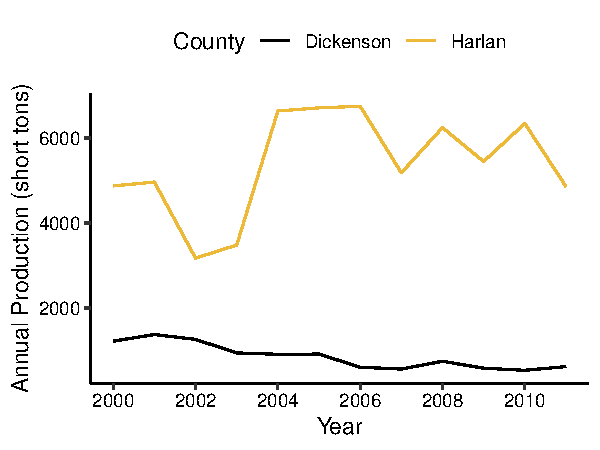
\includegraphics{Smith_ENV872_Project_files/figure-latex/unnamed-chunk-7-1.pdf}
\caption{\label{fig:figs} Total Annual Coal Production in Harlan and
Dickenson Counties}
\end{figure}

\hypertarget{question-2-is-the-number-of-people-employed-in-all-mines-in-the-boom-bust-county-harlan-in-the-years-2001-to-2011-significantly-greater-than-those-employed-by-a-bust-bust-county-dickenson-in-the-years-2001-to-2011}{%
\subsection{Question 2: Is the number of people employed in all mines in
the boom-bust county (Harlan) in the years 2001 to 2011 significantly
greater than those employed by a bust-bust county (Dickenson) in the
years 2001 to
2011?}\label{question-2-is-the-number-of-people-employed-in-all-mines-in-the-boom-bust-county-harlan-in-the-years-2001-to-2011-significantly-greater-than-those-employed-by-a-bust-bust-county-dickenson-in-the-years-2001-to-2011}}

\begin{Shaded}
\begin{Highlighting}[]
\NormalTok{employee <-}\StringTok{ }\KeywordTok{ggplot}\NormalTok{(minedata.clean, }\KeywordTok{aes}\NormalTok{(}\DataTypeTok{x =}\NormalTok{ year, }\DataTypeTok{y =}\NormalTok{ total.employee, }\DataTypeTok{color =}\NormalTok{ countystr)) }\OperatorTok{+}
\StringTok{  }\KeywordTok{geom_line}\NormalTok{() }\OperatorTok{+}
\StringTok{  }\KeywordTok{labs}\NormalTok{(}\DataTypeTok{x =} \StringTok{"Year"}\NormalTok{, }\DataTypeTok{y =} \StringTok{"Total Employed"}\NormalTok{, }\DataTypeTok{color =} \StringTok{"County"}\NormalTok{) }\OperatorTok{+}
\StringTok{  }\KeywordTok{xlim}\NormalTok{(}\DecValTok{2001}\NormalTok{, }\DecValTok{2011}\NormalTok{) }\OperatorTok{+}
\StringTok{  }\KeywordTok{scale_color_manual}\NormalTok{(}\DataTypeTok{values=}\NormalTok{hppal2) }\OperatorTok{+}
\StringTok{  }\KeywordTok{scale_x_continuous}\NormalTok{(}\StringTok{"Year"}\NormalTok{, }\KeywordTok{c}\NormalTok{(}\DecValTok{2001}\NormalTok{, }\DecValTok{2002}\NormalTok{, }\DecValTok{2003}\NormalTok{, }\DecValTok{2004}\NormalTok{, }\DecValTok{2005}\NormalTok{, }\DecValTok{2006}\NormalTok{, }\DecValTok{2007}\NormalTok{, }\DecValTok{2008}\NormalTok{, }\DecValTok{2009}\NormalTok{, }\DecValTok{2010}\NormalTok{, }\DecValTok{2011}\NormalTok{))}
\end{Highlighting}
\end{Shaded}

\begin{verbatim}
## Scale for 'x' is already present. Adding another scale for 'x', which will
## replace the existing scale.
\end{verbatim}

\begin{Shaded}
\begin{Highlighting}[]
\KeywordTok{print}\NormalTok{(employee)}
\end{Highlighting}
\end{Shaded}

\begin{verbatim}
## Warning: Removed 43 rows containing missing values (geom_path).
\end{verbatim}

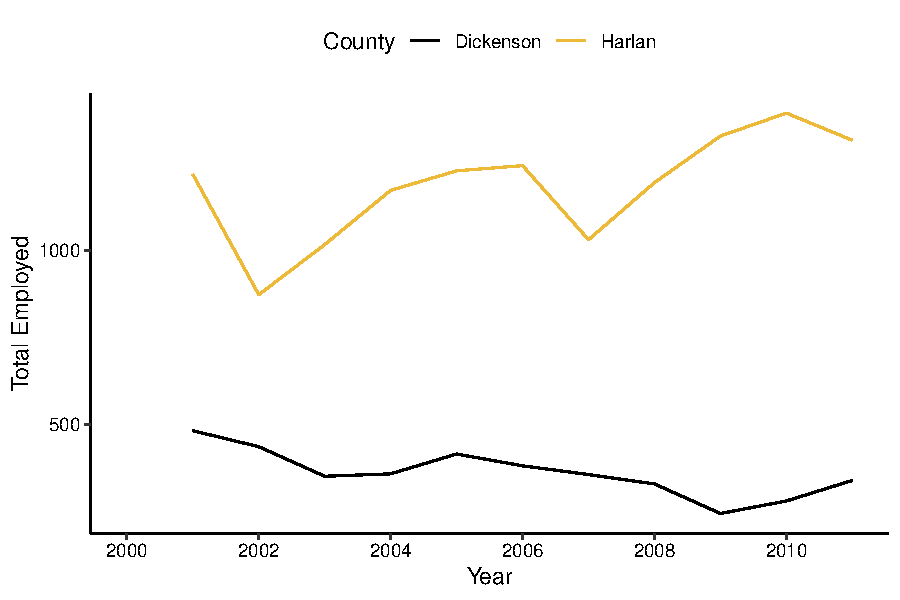
\includegraphics{Smith_ENV872_Project_files/figure-latex/unnamed-chunk-8-1.pdf}

\newpage

\hypertarget{summary-and-conclusions}{%
\section{Summary and Conclusions}\label{summary-and-conclusions}}

\newpage

\hypertarget{references}{%
\section{References}\label{references}}

\textless{}add references here if relevant, otherwise delete this
section\textgreater{}

\end{document}
